\documentclass[10pt,aspectratio=169]{beamer}
\usetheme{Madrid}
\usecolortheme{default}

\usepackage{tikz}
\usetikzlibrary{shapes.geometric, arrows.meta, positioning, calc}
\usepackage{booktabs}
\usepackage{array}
\usepackage{tabularx}
\usepackage{colortbl}
\usepackage{graphicx}
\usepackage{amsmath}

% --- COLOUR PALETTE ---
\definecolor{TLNavy}{HTML}{134E7C}
\definecolor{TLDivider}{HTML}{416B8A}
\definecolor{TLBlue}{HTML}{2375B7}
\definecolor{TLOrange}{HTML}{E07E19}
\definecolor{TLGreen}{HTML}{2E8B57}
\definecolor{TLRed}{HTML}{C0392B}
\definecolor{TLBlueBand}{HTML}{E9F2FA}
\definecolor{TLOrangeBand}{HTML}{FBE8D3}
\definecolor{HeaderNavy}{HTML}{13315C}
\definecolor{RowAlt}{HTML}{EEF3F8}

% --- FORMAT REQUIRED BY DEPARTMENT SAMPLE (First_Review_Sample_Presentation.pptx) ---
\setbeamertemplate{headline}{}
\setbeamertemplate{navigation symbols}{}
\setbeamercolor{footline}{fg=white,bg=TLNavy}
\setbeamertemplate{footline}{%
  \begin{beamercolorbox}[wd=\paperwidth,ht=2.6ex,dp=1.1ex,leftskip=0.35cm,rightskip=0.35cm]{footline}
    \scriptsize\sffamily First review - Final Year project \,\textbullet\, Team B17 \hfill Slide~\insertframenumber\,/\,\inserttotalframenumber
  \end{beamercolorbox}%
}

\title[Hierarchical Multi-Agent Sim -- Review 1]{Hierarchical Multi-Agent Population Simulation}
\author[Team B17]{Team B17}
\institute[Amrita]{School of Artificial Intelligence, Amrita Vishwa Vidyapeetham}
\date{}

\begin{document}

% ======================================================================
% SLIDE 1: TITLE SLIDE
% ======================================================================
\begin{frame}
\begin{center}
    {\large\bfseries\color{TLOrange} First review - Final Year project}\\[0.35cm]
    
\includegraphics[height=1.2cm]{amrita_logo.png}\\[0.35cm]
    {\Large\bfseries\color{TLNavy} Hierarchical Multi-Agent Population Simulation}\\[0.15cm]
    {\normalsize Calibrated Distribution-Valued Cluster Agents for Held-Out Survey Prediction}\\[0.45cm]
    {\small
    \textbf{Team No.:} B17\\[0.2cm]
    \begin{tabular}{ll}
    Nitin Krishna V & CB.SC.U4AIE23156 \\
    Vishal S & CB.SC.U4AIE23160 \\
    Manogna Challa & CB.SC.U4AIE23175 \\
    Gaurav Mahesh & CB.SC.U4AIE23176 \\
    \end{tabular}\\[0.25cm]
    \textbf{Mentor:} Dr. Snigdhatanu Acharya \qquad \textbf{Co-Mentor:} Dr. Premjith B.\\[0.15cm]
    School of Artificial Intelligence, Amrita Vishwa Vidyapeetham
    }
\end{center}
\end{frame}

% ======================================================================
% SLIDE 2: 01 | PROJECT PROGRESS SINCE ZEROTH REVIEW
% ======================================================================
\begin{frame}{01 | Project Progress Since Zeroth Review}
    \small
    \textbf{Core focus of Review 1:} Show what has been \textbf{built, tested, and validated} on real microdata since Zeroth Review.

    \vspace{0.15cm}
    \begin{columns}[T]
        \begin{column}{0.48\textwidth}
            \begin{block}{What We Built \& Verified}
                \scriptsize
                \begin{itemize}\itemsep3pt
                    \item Built the full \textbf{M1--M10 pipeline} (174 automated tests passing, 0 lint warnings).
                    \item Evaluated the pre-registered claim end-to-end on \textbf{pooled GSS 2010--2022} ($n=18{,}772$) across 3 models (3B, 8B, 14B).
                    \item \textbf{14B result:} $-25.3\%$ error reduction over national baseline (beating our pre-registered $-20\%$ target).
                    \item True population variance recovered (ratio \textbf{1.009}, target $[0.8, 1.2]$).
                \end{itemize}
            \end{block}
        \end{column}
        \begin{column}{0.52\textwidth}
            \begin{block}{Where Real Data Corrected Our Initial Spec}
                \tiny
                \renewcommand{\arraystretch}{1.15}
                \begin{tabularx}{\textwidth}{@{} >{\raggedright\arraybackslash}p{2.3cm} >{\raggedright\arraybackslash}p{1.7cm} X @{}}
                    \toprule
                    \rowcolor{HeaderNavy} \textcolor{white}{\textbf{Parameter}} & \textcolor{white}{\textbf{Initial Spec}} & \textcolor{white}{\textbf{Measured Reality}} \\
                    \midrule
                    \rowcolor{RowAlt} Cluster count & $K = 150$ & \textbf{$K = 56$} ($\ge 60$ respondents/cell) \\
                    Dataset bed & GSS 2024 & \textbf{Pooled 2010--2022} (2024 missing region) \\
                    \rowcolor{RowAlt} Partition axes & Demo + Geo & \textbf{Age $\times$ Degree $\times$ Sex} (geo in stat card) \\
                    Usable items & 148 items & \textbf{74 items} clear SNR $\ge 1.5$ gate \\
                    \rowcolor{RowAlt} Compute budget & \$1,200 & \textbf{\$0} (Free tiers + cache + router) \\
                    \bottomrule
                \end{tabularx}
            \end{block}
        \end{column}
    \end{columns}
\end{frame}

% ======================================================================
% SLIDE 3: 02 | MOTIVATION & PROBLEM STATEMENT
% ======================================================================
\begin{frame}{02 | Motivation \& Problem Statement}
    \small
    \textbf{Problem:} Given a demographic group described only by population shares and answers to a set of \emph{other} survey questions, what is the full response \textbf{distribution} (histogram) to an unasked question?

    \vspace{0.15cm}
    \begin{columns}[T]
        \begin{column}{0.48\textwidth}
            \begin{block}{Why Distributions \& Clusters?}
                \scriptsize
                \begin{itemize}\itemsep3pt
                    \item \textbf{Means hide polarization:} An average score of 2.5 on a 5-point scale cannot tell apart consensus from extreme polarization.
                    \item \textbf{Persona collapse (F1/F2):} Querying individual agents collapses variance within groups and regresses between groups.
                    \item \textbf{Cross-tabs are static:} Real surveys cannot answer questions they never asked.
                \end{itemize}
            \end{block}
            \vspace{0.05cm}
            \scriptsize \textbf{Scope:} US General Social Survey (pooled 2010--2022, primary); India Global Flourishing Study ($n=12{,}765$, secondary replication).
        \end{column}
        \begin{column}{0.52\textwidth}
            \begin{block}{Pre-Registered Objectives (Fixed in Advance)}
                \scriptsize
                \begin{itemize}\itemsep4pt
                    \item \textbf{Objective 1 (Accuracy):} Beat the national-marginal baseline (B0a) by $\ge 20\%$ Wasserstein-1 ($W_1$) error on held-out questions where subgroups genuinely differ.
                    \item \textbf{Objective 2 (Distributional Shape):} Recover true population variance ratio within $[0.8, 1.2]$ (solving variance collapse).
                    \item \textbf{Objective 3 (Efficiency):} Match per-individual persona sampling at equal or lower query budget (\$0 cost via free tiers).
                \end{itemize}
            \end{block}
        \end{column}
    \end{columns}
\end{frame}

% ======================================================================
% SLIDE 4: 03 | CONSOLIDATED LITERATURE REVIEW & RESEARCH GAP
% ======================================================================
\begin{frame}{03 | Consolidated Literature Review \& Research Gap}
    \scriptsize
    \renewcommand{\arraystretch}{1.15}
    \begin{table}
        \centering
        \begin{tabularx}{\textwidth}{@{} >{\raggedright\arraybackslash}p{2.6cm} >{\raggedright\arraybackslash}X >{\raggedright\arraybackslash}X @{}}
            \toprule
            \rowcolor{HeaderNavy}
            \textcolor{white}{\textbf{Paper}} & \textcolor{white}{\textbf{Key Finding}} & \textcolor{white}{\textbf{Identified Limitation}} \\
            \midrule
            \rowcolor{RowAlt} Argyle et al. (2023) & GPT-3 personas track human response patterns. & Static; no distributional calibration. \\
            Bisbee et al. (2024) & Persona-prompted LLMs track human averages. & Severe variance collapse within subgroups (F1). \\
            \rowcolor{RowAlt} Santurkar et al. (2023) & OpinionQA benchmark across Pew surveys. & Measures national steering, lacks subgroup calibration. \\
            Park et al. (2023, 2024) & Generative agents / 1,000 interview-grounded agents. & Linear compute scaling (1 agent / person); flat population. \\
            \rowcolor{RowAlt} Li et al. (2024) / Pi et al. (2025) & EconAgent, AgentSociety: large-scale multi-agent sim. & Heavy compute; homogeneous personas without shrinkage. \\
            \bottomrule
        \end{tabularx}
    \end{table}

    \vspace{0.1cm}
    \begin{columns}[T]
        \begin{column}{0.33\textwidth}
            \begin{block}{\scriptsize Gap 1: Compute Cost}
                \tiny Simulating 10,000s of individuals is prohibitively expensive. \\
                \textbf{Our Fix:} 1 query per demographic cluster ($K=56$).
            \end{block}
        \end{column}
        \begin{column}{0.33\textwidth}
            \begin{block}{\scriptsize Gap 2: Variance Collapse}
                \tiny Persona prompting collapses within-group spread. \\
                \textbf{Our Fix:} Elicit full histograms + cross-fitted anchor calibration.
            \end{block}
        \end{column}
        \begin{column}{0.33\textwidth}
            \begin{block}{\scriptsize Gap 3: Statistical Hierarchy}
                \tiny Flat agent pools lack structured group dynamics. \\
                \textbf{Our Fix:} Supervised tree partial pooling + subspace projection.
            \end{block}
        \end{column}
    \end{columns}
\end{frame}

% ======================================================================
% SLIDE 5: 04 | FINALIZED SYSTEM ARCHITECTURE & METHODOLOGY
% ======================================================================
\begin{frame}{04 | Finalized System Architecture \& Methodology}
    \centering
    \resizebox{0.92\textwidth}{!}{%
    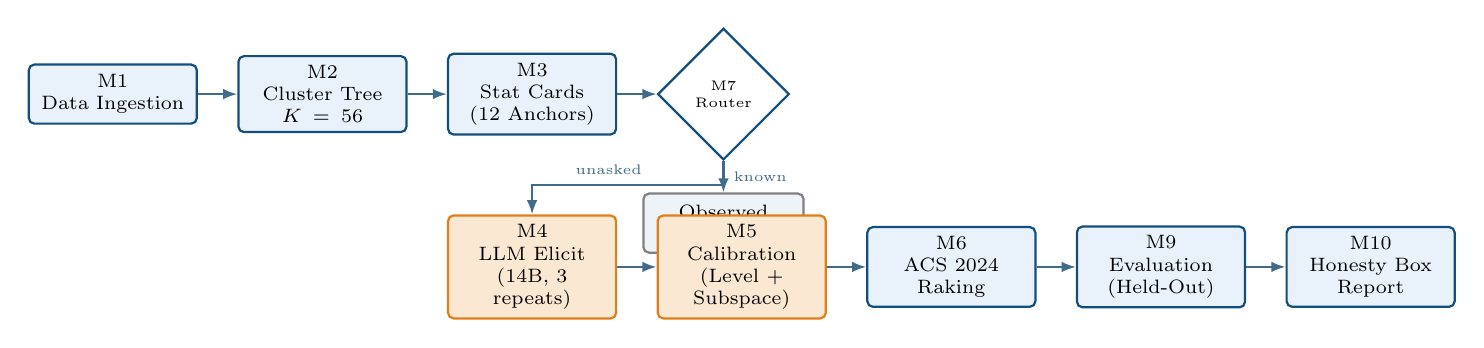
\begin{tikzpicture}[
        node distance=4mm and 5mm,
        every node/.style={font=\scriptsize},
        block/.style={rectangle, rounded corners=2pt, draw=TLNavy, fill=TLBlueBand, text width=1.9cm, align=center, minimum height=0.75cm, thick},
        core/.style={block, fill=TLOrangeBand, draw=TLOrange},
        obsstyle/.style={block, fill=RowAlt, draw=gray, text width=1.8cm},
        diam/.style={diamond, draw=TLNavy, fill=white, text width=1.2cm, align=center, minimum height=0.75cm, thick, font=\tiny, inner sep=1pt},
        arr/.style={-{Latex[length=1.8mm]}, thick, TLDivider}
    ]
        \node[block] (m1) {M1\\Data Ingestion};
        \node[block, right=of m1] (m2) {M2\\Cluster Tree\\$K=56$};
        \node[block, right=of m2] (m3) {M3\\Stat Cards\\(12 Anchors)};
        \node[diam, right=of m3] (m7) {M7\\Router};
        \node[obsstyle, below=of m7] (obs) {Observed\\Cross-tab};

        \node[core, below=10mm of m3] (m4) {M4\\LLM Elicit\\(14B, 3 repeats)};
        \node[core, right=of m4] (m5) {M5\\Calibration\\(Level + Subspace)};
        \node[block, right=of m5] (m6) {M6\\ACS 2024\\Raking};
        \node[block, right=of m6] (m9) {M9\\Evaluation\\(Held-Out)};
        \node[block, right=of m9] (m10) {M10\\Honesty Box\\Report};

        \draw[arr] (m1) -- (m2);
        \draw[arr] (m2) -- (m3);
        \draw[arr] (m3) -- (m7);
        \draw[arr] (m7.south) -- ++(0,-0.3) -| node[pos=0.3, above, font=\tiny]{unasked} (m4.north);
        \draw[arr] (m7) -- node[right, font=\tiny]{known} (obs);
        \draw[arr] (m4) -- (m5);
        \draw[arr] (m5) -- (m6);
        \draw[arr] (m6) -- (m9);
        \draw[arr] (m9) -- (m10);
    \end{tikzpicture}%
    }

    \vspace{0.15cm}
    \scriptsize
    \textbf{Mathematical Formulation (Level/Structure Decomposition):}
    \[
        \text{pred\_cdf}(c) \;=\; \underbrace{\text{level\_cdf}}_{\text{national topline}} \;+\; s \cdot \underbrace{P_r}_{\text{subspace projection}} \underbrace{\Big(\text{raw\_cdf}(c) - {\textstyle\sum_c} w_c\, \text{raw\_cdf}(c)\Big)}_{\text{model's subgroup deviation}}
    \]
    \begin{itemize}\itemsep2pt
        \item \textbf{M7 Oracle Router:} If a question is already in the GSS, it returns the weighted cross-tab directly (\$0 cost, 0 error). The LLM is invoked \textbf{only} for unasked questions.
        \item \textbf{Calibration on Anchors Only:} Scale $s$ and projection $P_r$ are fitted on 34 anchors via $F=3$ cross-fitting. No target truth is ever touched.
    \end{itemize}
\end{frame}

% ======================================================================
% SLIDE 6: 05 | IMPLEMENTATION STATUS – PROTOTYPE / PROOF-OF-CONCEPT
% ======================================================================
\begin{frame}{05 | Implementation Status -- Prototype / Proof-of-Concept}
    \scriptsize
    \begin{columns}[T]
        \begin{column}{0.5\textwidth}
            \renewcommand{\arraystretch}{1.1}
            \begin{table}
            \begin{tabularx}{\textwidth}{@{} >{\raggedright\arraybackslash}X c @{}}
                \toprule
                \rowcolor{HeaderNavy} \textcolor{white}{\textbf{Pipeline Module}} & \textcolor{white}{\textbf{Status}} \\
                \midrule
                \rowcolor{RowAlt} M1 Data Ingestion \& Harmonization & {\color{TLGreen}\textbf{Done}} \\
                M2 Cluster Tree \& Sampling Noise & {\color{TLGreen}\textbf{Done}} \\
                \rowcolor{RowAlt} M3 Stat Card Builder & {\color{TLGreen}\textbf{Done}} \\
                M4 LLM Distributional Elicitation & {\color{TLGreen}\textbf{Done}} \\
                \rowcolor{RowAlt} M5 Cross-Fitted Calibration & {\color{TLGreen}\textbf{Done}} \\
                M6 Post-Stratification Raking & {\color{TLGreen}\textbf{Done}} \\
                \rowcolor{RowAlt} M7 Oracle Router (TF-IDF Cosine) & {\color{TLGreen}\textbf{Done}} \\
                M8 Opinion Dynamics & {\color{TLOrange}\textbf{Stage B}} \\
                \rowcolor{RowAlt} M9 Evaluation Harness & {\color{TLGreen}\textbf{Done}} \\
                M10 Streamlit App + Honesty Box & {\color{TLGreen}\textbf{Done}} \\
                \bottomrule
            \end{tabularx}
            \end{table}
        \end{column}
        \begin{column}{0.5\textwidth}
            \begin{block}{Software Verification \& Quality}
                \scriptsize
                \begin{itemize}\itemsep4pt
                    \item \textbf{174 automated tests passing} with \texttt{pytest}; 0 lint errors.
                    \item \textbf{Free-tier infrastructure:} Multi-provider router (Mistral, Groq, Gemini) with per-provider daily quotas and call-count guards.
                    \item \textbf{Atomic SQLite caching:} Every call cached by prompt hash; pipeline can be halted and resumed without losing state.
                    \item \textbf{Two independent verifications}: Re-derived macro $W_1$ ($0.00\mathrm{e}{+}00$ diff) and verified 1,147/1,148 published GSS codebook tables.
                \end{itemize}
            \end{block}
        \end{column}
    \end{columns}
\end{frame}

% ======================================================================
% SLIDE 7: 06 | EXPERIMENTAL SETUP & TEST CASES
% ======================================================================
\begin{frame}{06 | Experimental Setup \& Test Cases}
    \scriptsize
    \begin{columns}[T]
        \begin{column}{0.48\textwidth}
            \textbf{Dataset Bed \& Partitioning:}
            \begin{itemize}\itemsep3pt
                \item \textbf{GSS pooled 2010--2022} ($n = 18{,}772$ respondents).
                \item Partition: \texttt{age\_band} $\times$ \texttt{degree} $\times$ \texttt{sex} $\implies$ \textbf{$K=56$} clusters (min cell size 60).
                \item \textbf{Split-half noise gate:} 74 of 148 items cleared SNR $\ge 1.5$ (sampling noise floor = 0.0273).
                \item \textbf{Frozen split:} 34 anchors / 40 targets (39 scored), topic-stratified, persisted to disk.
                \item \textbf{ACS 2024 PUMS raking:} 60 cells, 267.2M US adults (validated against GSS within 2.9 pp).
                \item \textbf{Models:} Ministral 3B, 8B (development), 14B (headline) via free APIs (\$0 cost).
            \end{itemize}
        \end{column}
        \begin{column}{0.52\textwidth}
            \textbf{Six Verification Layers (Pre-Registered Gates):}
            \renewcommand{\arraystretch}{1.15}
            \begin{table}
            \begin{tabularx}{\textwidth}{@{} c >{\raggedright\arraybackslash}X c @{}}
                \toprule
                \rowcolor{HeaderNavy} \textcolor{white}{\textbf{Gate}} & \textcolor{white}{\textbf{Verification Check}} & \textcolor{white}{\textbf{Result}} \\
                \midrule
                \rowcolor{RowAlt} L0 & Published GSS topline matching & {\color{TLGreen}\textbf{PASS}} (142/142 $\le$0.5pp) \\
                L1 & Ground truth noise floor estimation & {\color{TLGreen}\textbf{PASS}} (floor 0.0273) \\
                \rowcolor{RowAlt} L2 & Permutation test (card-shuffling) & {\color{TLGreen}\textbf{PASS}} (+0.0689 gap) \\
                L3 & Calibration oracle round-trip & {\color{TLGreen}\textbf{PASS}} ($1.1\times 10^{-16}$) \\
                \rowcolor{RowAlt} L4 & Held-out targets vs baseline B0a & {\color{TLGreen}\textbf{PASS}} ($-25.3\%$) \\
                L5 & Direct memorization / leakage probe & {\color{TLGreen}\textbf{PASS}} (2/39 flagged) \\
                \bottomrule
            \end{tabularx}
            \end{table}
            \tiny \textbf{Strict Rule:} Layers 0--2 were enforced as hard build gates before any downstream calibration was executed.
        \end{column}
    \end{columns}
\end{frame}

% ======================================================================
% SLIDE 8: 07 | RESULTS – QUANTITATIVE PERFORMANCE
% ======================================================================
\begin{frame}{07 | Results -- Quantitative Performance}
    \scriptsize
    \textbf{Evaluated on 39 held-out targets $\times$ 56 clusters using Ministral 14B (12,540 elicitations).} \\
    \textbf{Honest 3-Number Reporting:} Achieved $W_1$, Baseline B0a, and Noise Floor reported together.
    \vspace{0.1cm}

    \renewcommand{\arraystretch}{1.18}
    \begin{table}
    \begin{tabularx}{\textwidth}{@{} >{\raggedright\arraybackslash}X c c c c c @{}}
        \toprule
        \rowcolor{HeaderNavy}
        \textcolor{white}{\textbf{Item Subset}} & \textcolor{white}{\textbf{Achieved $W_1$}} & \textcolor{white}{\textbf{Baseline B0a}} & \textcolor{white}{\textbf{Floor}} & \textcolor{white}{\textbf{Absolute Mark}} & \textcolor{white}{\textbf{Relative Gain ($-20\%$)}} \\
        \midrule
        \rowcolor{RowAlt} \textbf{All 39 held-out targets} & \textbf{0.0602} & 0.0807 & 0.0273 & $\le 0.0556$ (fail) & {\color{TLGreen}\textbf{PASS ($-25.3\%$)}} \\
        \textbf{Top-quartile heterogeneity} & \textbf{0.0787} & 0.1139 & 0.0402 & $\le 0.0834$ ({\color{TLGreen}\textbf{PASS}}) & {\color{TLGreen}\textbf{PASS ($-30.9\%$)}} \\
        \rowcolor{RowAlt} \textbf{Leakage-resistant subset} & \textbf{0.0565} & 0.0757 & 0.0324 & $\le 0.0614$ ({\color{TLGreen}\textbf{PASS}}) & {\color{TLGreen}\textbf{PASS ($-25.4\%$)}} \\
        Uncalibrated LLM (B4) & 0.1926 & 0.0807 & 0.0273 & -- & \textbf{Calibration cuts error 69\%} \\
        \bottomrule
    \end{tabularx}
    \end{table}

    \vspace{0.1cm}
    \begin{columns}[T]
        \begin{column}{0.48\textwidth}
            \begin{block}{Objective 2: Variance \& Calibration}
                \tiny
                \begin{itemize}\itemsep2pt
                    \item \textbf{Population variance ratio: 1.009} (within $[0.8, 1.2]$ band $\implies$ Objective 2 passed).
                    \item \textbf{90\% interval coverage: 0.899} (matches nominal 0.90).
                    \item \textbf{Tolerance battery ordering: $\rho = +0.879$} across 5 target groups.
                \end{itemize}
            \end{block}
        \end{column}
        \begin{column}{0.52\textwidth}
            \begin{block}{Model Scaling: Capability Curve}
                \tiny
                \begin{itemize}\itemsep2pt
                    \item \textbf{Ministral 3B:} $W_1 = 0.0686$ ($-15.0\%$ vs baseline).
                    \item \textbf{Ministral 8B:} $W_1 = 0.0634$ ($-21.4\%$ vs baseline).
                    \item \textbf{Ministral 14B:} $W_1 = 0.0602$ ($-25.3\%$ vs baseline).
                    \item \textbf{Takeaway:} Error decreases monotonically with model size.
                \end{itemize}
            \end{block}
        \end{column}
    \end{columns}
\end{frame}

% ======================================================================
% SLIDE 9: 08 | RESULTS ANALYSIS & INTERPRETATION
% ======================================================================
\begin{frame}{08 | Results Analysis \& Interpretation}
    \scriptsize
    \begin{columns}[T]
        \begin{column}{0.5\textwidth}
            \begin{block}{The Big Finding: Error Decomposition}
                \tiny
                \begin{itemize}\itemsep3pt
                    \item Raw LLM error ($\approx 0.20$ $W_1$) is \textbf{not} caused by collapsed subgroup differences.
                    \item It is dominated by a \textbf{constant per-item level offset} (e.g., predicting 0.72 on \texttt{spkcom} when true average is 0.29).
                    \item \textbf{Subgroup ranking is already present:} Between-cluster Spearman $\rho = \mathbf{+0.597}$ macro on 14B (8 of 10 items statistically significant).
                    \item \textbf{Gate 3 explained:} Raw card permutation was red (+0.0011) because raw $W_1$ was swamped by the level error. Once level-matched, real vs permuted gap was \textbf{+0.0689} (green).
                \end{itemize}
            \end{block}
        \end{column}
        \begin{column}{0.5\textwidth}
            \begin{block}{Ablations: What Is Load-Bearing?}
                \tiny
                \begin{itemize}\itemsep3pt
                    \item \textbf{Subspace Projection ($P_r$):} Restricting deviations to top anchor directions cuts error from 0.0688 to 0.0638 ($-7\%$ gain).
                    \item \textbf{Topic Transfer:} Standard vs adversarial topic-disjoint calibration is 0.0638 vs 0.0641 (only 0.0003 cost $\implies$ anchors transfer across topics).
                    \item \textbf{Stat-Card Anchors:} Adding 12 anchors improves over demographics alone by $-6.8\%$.
                    \item \textbf{Item Win Rate:} System beats national baseline on \textbf{36 of 39} items. The 3 losses are flat spending items (\texttt{natroad}, \texttt{natarms}, \texttt{natmass}).
                \end{itemize}
            \end{block}
        \end{column}
    \end{columns}
\end{frame}

% ======================================================================
% SLIDE 10: 09 | PROTOTYPE / DEMONSTRATION
% ======================================================================
\begin{frame}{09 | Prototype / Demonstration}
    \small
    \textbf{Working Prototype:} \texttt{simulate\_region.py} and Streamlit application (\texttt{M10\_app}).

    \vspace{0.15cm}
    \begin{columns}[T]
        \begin{column}{0.5\textwidth}
            \begin{block}{Dual-Path Query Routing}
                \scriptsize
                \begin{itemize}\itemsep4pt
                    \item \textbf{Observed Survey Query:} If the query matches a GSS item (e.g. \texttt{satfin}), the router serves the weighted cross-tab instantly (0 LLM calls, 0 cost, exact ground truth).
                    \item \textbf{Unasked Policy Scenario:} Elicits distributions across the 56 cluster agents, applies anchor calibration, and rakes to ACS census weights.
                \end{itemize}
            \end{block}
        \end{column}
        \begin{column}{0.5\textwidth}
            \begin{block}{The Lead Demo \& The Honesty Box}
                \scriptsize
                \begin{itemize}\itemsep4pt
                    \item \textbf{Demo item:} \texttt{natroad} (highway/bridge spending) -- clean demographic gradient (SNR 3.61), not over-debated in public media.
                    \item \textbf{Mandatory Honesty Box:} Every prediction is displayed alongside:
                    \begin{enumerate}\tiny\itemsep1pt
                        \item The nearest validated held-out survey item.
                        \item Its measured $W_1$ score and baseline distance.
                    \end{enumerate}
                    \item Prevents overclaiming on synthetic policy scenarios where ground truth does not exist.
                \end{itemize}
            \end{block}
        \end{column}
    \end{columns}
\end{frame}

% ======================================================================
% SLIDE 11: 10 | CURRENT LIMITATIONS & TECHNICAL CHALLENGES
% ======================================================================
\begin{frame}{10 | Current Limitations \& Technical Challenges}
    \scriptsize
    \begin{columns}[T]
        \begin{column}{0.5\textwidth}
            \begin{block}{Engineering Challenges Solved}
                \tiny
                \begin{itemize}\itemsep4pt
                    \item \textbf{Free-tier rate limits:} Ministral 14B was capped at 30 req/min $\implies$ implemented provider failover, request pacing, and daily token budget guards.
                    \item \textbf{Shell execution timeouts:} Long batch runs were split into atomic checkpoints; prompt-hash SQLite cache ensures zero repeated spend.
                    \item \textbf{GSS 2024 data defect:} Discovered that 2024 release had 0\% populated \texttt{region\_7222} $\implies$ pivoted to pooled 2010--2022 rather than corrupting the partition.
                    \item \textbf{Groq sandbox block:} Groq was blocked by Cloudflare in the cloud sandbox $\implies$ developed fallback routing to Mistral/Gemini.
                \end{itemize}
            \end{block}
        \end{column}
        \begin{column}{0.5\textwidth}
            \begin{block}{Known Scientific Limitations}
                \tiny
                \begin{itemize}\itemsep4pt
                    \item \textbf{Conservative between-cluster spread:} The system captures cluster ordering ($\rho = +0.651$), but between-cluster SD is $\approx 2\times$ conservative (predicted 0.0550 vs true 0.0979) due to $W_1$-minimizing shrinkage ($s < 1$).
                    \item \textbf{Single country tested so far:} US GSS is complete; India replication on GFS is staged but not yet evaluated.
                    \item \textbf{Fixed prompt phrasing:} Current runs use 1 paraphrase $\times$ 3 repeats; testing robustness across 3 distinct paraphrases is slated for Stage B.
                \end{itemize}
            \end{block}
        \end{column}
    \end{columns}
\end{frame}

% ======================================================================
% SLIDE 12: 11 | REMAINING WORK & COMPLETION PLAN
% ======================================================================
\begin{frame}{11 | Remaining Work \& Completion Plan}
    \small
    \textbf{Stage B Execution Plan (Roadmap to Final Review):}

    \vspace{0.15cm}
    \begin{columns}[T]
        \begin{column}{0.5\textwidth}
            \begin{block}{Stage B Experimental Tasks}
                \scriptsize
                \begin{itemize}\itemsep3pt
                    \item \textbf{India Replication:} Run pipeline on Global Flourishing Study (GFS, $n=12{,}765$, `COUNTRY=6`).
                    \item \textbf{Cross-Instrument Generalization:} Evaluate on Pew OpinionQA (15 ATP waves).
                    \item \textbf{Paraphrase-Axis Ensemble:} Evaluate sensitivity across 3 hand-written question paraphrases.
                    \item \textbf{Opinion Dynamics (M8):} Model attitude shifts across repeated cross-sections with time horizon as a variable.
                \end{itemize}
            \end{block}
        \end{column}
        \begin{column}{0.5\textwidth}
            \begin{block}{Target Deliverables \& Timeline}
                \scriptsize
                \begin{itemize}\itemsep3pt
                    \item \textbf{Weeks 1--4:} Complete GFS India run and cross-instrument OpinionQA evaluation.
                    \item \textbf{Weeks 5--7:} Implement M8 opinion dynamics on historical GSS waves.
                    \item \textbf{Weeks 8--10:} Deploy finalized Streamlit decision dashboard with US and India scenario walkthroughs.
                    \item \textbf{Weeks 11--12:} Thesis documentation and manuscript finalization for conference submission.
                \end{itemize}
            \end{block}
        \end{column}
    \end{columns}
\end{frame}

% ======================================================================
% SLIDE 13: 12 | PROJECT CONTRIBUTION & CURRENT ACHIEVEMENT
% ======================================================================
\begin{frame}{12 | Project Contribution \& Current Achievement}
    \scriptsize
    \begin{block}{Defensible Project Contributions}
        \tiny
        \begin{enumerate}\itemsep3pt
            \item \textbf{Distributional Cluster-Agent Framework:} Represents populations via interpretable demographic clusters ($K=56$) rather than expensive flat agents, recovering true population variance (ratio 1.009).
            \item \textbf{Level/Structure Calibration:} Solves LLM bias by separating national level offsets from true subgroup variation using out-of-fold anchor questions.
            \item \textbf{Pre-Registered 6-Layer Falsification Protocol:} Every claim evaluated against hard baselines (B0a) and sampling noise floors with independent verification ($0.00\mathrm{e}{+}00$ discrepancy).
        \end{enumerate}
    \end{block}

    \vspace{0.1cm}
    \begin{columns}[T]
        \begin{column}{0.5\textwidth}
            \begin{block}{6 Empirical Corrections to the Proposal}
                \tiny
                \begin{itemize}\itemsep2pt
                    \item Corrected $K=150 \to 56$ based on cell noise floor.
                    \item Replaced GSS 2024 with pooled 2010--2022.
                    \item Replaced \$1,200 budget with \$0 free-tier router.
                    \item Tuned router cosine threshold $0.85 \to 0.25$ (recall $0 \to 81\%$).
                    \item Restricted subspace projection to active clusters.
                    \item Dropped counter-productive variance expansion.
                \end{itemize}
            \end{block}
        \end{column}
        \begin{column}{0.5\textwidth}
            \begin{block}{Claims We Explicitly Do NOT Make}
                \tiny
                \begin{itemize}\itemsep2pt
                    \item \textbf{Not} ``simulating human consciousness or entire societies''.
                    \item \textbf{Not} ``predicting real-world election outcomes''.
                    \item \textbf{Not} claiming ground-truth accuracy on unvalidated policy scenarios (addressed by the Honesty Box).
                    \item We claim: \textbf{Accurately recovering held-out subgroup survey distributions where subgroups genuinely differ.}
                \end{itemize}
            \end{block}
        \end{column}
    \end{columns}
\end{frame}

% ======================================================================
% SLIDE 14: 13 | TEAM CONTRIBUTION & RESPONSIBILITY
% ======================================================================
\begin{frame}{13 | Team Contribution \& Responsibility}
    \small
    \begin{columns}[T]
        \begin{column}{0.48\textwidth}
            \begin{block}{Vishal S (CB.SC.U4AIE23160)}
                \scriptsize
                \textbf{Role:} Data Ingestion \& Clustering Lead \\
                \textbf{Completed Modules:}
                \begin{itemize}\itemsep1pt
                    \item M1 Data Ingestion \& Harmonization (GSS pooled adapter)
                    \item M2 Cluster Tree ($K=56$) \& Kish Effective $N$
                    \item Layer 0 Published Codebook Topline Verification
                \end{itemize}
            \end{block}
            \vspace{0.1cm}
            \begin{block}{Nitin Krishna V (CB.SC.U4AIE23156)}
                \scriptsize
                \textbf{Role:} Agent Design Lead \\
                \textbf{Completed Modules:}
                \begin{itemize}\itemsep1pt
                    \item M3 Stat Card Generator \& Fold Isolation Contract
                    \item M4 Distributional Elicitation Runner \& Schemas
                    \item Multi-provider API router \& SQLite cache integration
                \end{itemize}
            \end{block}
        \end{column}
        \begin{column}{0.48\textwidth}
            \begin{block}{Gaurav Mahesh (CB.SC.U4AIE23176)}
                \scriptsize
                \textbf{Role:} Simulation \& Integration Lead \\
                \textbf{Completed Modules:}
                \begin{itemize}\itemsep1pt
                    \item M5 Cross-Fitted Calibration (Level + Subspace)
                    \item M6 Post-Stratification Raking (ACS 2024 PUMS)
                    \item Layer 2 Permutation Test \& Gate 3 Diagnosis
                \end{itemize}
            \end{block}
            \vspace{0.1cm}
            \begin{block}{Manogna Challa (CB.SC.U4AIE23175)}
                \scriptsize
                \textbf{Role:} Analytics \& Visualization Lead \\
                \textbf{Completed Modules:}
                \begin{itemize}\itemsep1pt
                    \item M9 Evaluation Metric Harness ($W_1$, JS, ECE, Coverage)
                    \item M10 Streamlit Application \& Mandatory Honesty Box
                    \item Layer 5 Leakage \& Direct Recall Probing
                \end{itemize}
            \end{block}
        \end{column}
    \end{columns}
\end{frame}

% ======================================================================
% SLIDE 15: 14 | REFERENCES
% ======================================================================
\begin{frame}{14 | References}
    \footnotesize
    \begin{thebibliography}{99}
        \bibitem{argyle2023} L. P. Argyle et al., ``Out of One, Many: Using Language Models to Simulate Human Samples,'' \textit{Political Analysis}, 2023.
        \bibitem{bisbee2024} J. Bisbee et al., ``The Perils of Using Large Language Models to Replace Human Participants,'' \textit{Political Analysis}, 2024.
        \bibitem{santurkar2023} S. Santurkar et al., ``Whose Opinions Do Language Models Reflect?,'' \textit{ICML (OpinionQA)}, 2023.
        \bibitem{kull2019} M. Kull et al., ``Beyond Temperature Scaling: Obtaining Well-Calibrated Multi-Class Probabilities with Dirichlet Calibration,'' \textit{NeurIPS}, 2019.
        \bibitem{park2023} J. S. Park et al., ``Generative Agents: Interactive Simulacra of Human Behavior,'' \textit{ACM UIST}, 2023.
        \bibitem{park2024} J. S. Park et al., ``Generative Agent Simulations of 1,000 People,'' \textit{arXiv:2411.10109}, 2024.
        \bibitem{li2024} Y. Li et al., ``EconAgent: Large Language Model-Empowered Agents for Simulating Macroeconomic Activities,'' \textit{ACL}, 2024.
        \bibitem{pi2025} X. Pi et al., ``AgentSociety: Large-Scale Simulation of Agent Societies,'' \textit{arXiv:2502.08601}, 2025.
        \bibitem{chopra2025} S. Chopra et al., ``Large-Scale LLM-Archetype Agent-Based Modeling,'' 2025.
    \end{thebibliography}
\end{frame}

\end{document}
